\ifx\wholebook\relax \else

\documentclass{article}

\usepackage[nomarginpar
  %, margin=.5in
]{geometry}

\addtolength{\oddsidemargin}{-0.05in}
\addtolength{\evensidemargin}{-0.05in}
\addtolength{\textwidth}{0.1in}

\usepackage[en]{../prelude}

\setcounter{page}{1}

\begin{document}

\title{Fusion}

\author{Liu Xinyu
\thanks{{\bfseries Liu Xinyu} \newline
  Email: liuxinyu95@gmail.com \newline}
  }

\maketitle
\fi

\markboth{Fusion}{Mathematics of Programming}

\ifx\wholebook\relax
\chapter{Fusion}
\numberwithin{Exercise}{chapter}
\fi

\epigraph{... mathematical knowledge ... is, in fact, merely verbal knowledge. ``3'' means ``2+1'', and ``4'' means ``3+1''. Hence it follows (though the proof is long) that ``4'' means the same as ``2+2''. Thus mathematical knowledge ceases to be mysterious.}{-- Bertrand Russell}

\begin{wrapfigure}{R}{0.4\textwidth}
 \centering
 \includegraphics[scale=0.5]{img/penrose-triangle.png}
 \captionsetup{labelformat=empty}
 \caption{Penrose triangle}
 \label{fig:Penrose-triangle}
\end{wrapfigure}

I still remember the mathematics class in high school. My teacher often wrote down a complex formula with many alphabetic symbols in the blackboard, then asked us to simplify it. Some student stood up, volunteered to do it in front of the class. Combining like terms, factorization, ... all means were attempted. It liked a magic process often led to unbelievable simple result. Of course sometimes the guy was stuck or trapped in loops, and finally saved by our teacher.

Chalk and blackboard, Such experience was unforgettable, just like happened yesterday. I was so impressed to the mythical power of reasoning. I always wanted to know more formulas, that could help me to deduce the result.

The magic is that, we even needn't care about the concrete meanings when doing the deduction. It likes building bricks, from different parts, we finally build an interesting toy. These formulas and theorems can also be combined together, and finally build an interesting result. When meet $a^2 + 2ab + b^2$, then turn it into $(a+b)^2$, just like mating two bricks. We needn't force ourselves to remind the geometric meanings for this formula when deducing it.

\begin{figure}[htbp]
\centering
\begin{tikzpicture}
\draw[fill=gray, draw=black, pattern=north west lines]
  (0, 0) rectangle (4, 4);
\filldraw[fill=white]
  (0, 0) rectangle (1, 1)
  (1, 1) rectangle (4, 4);
\path (0.5, 0.5) node {$a^2$}
      (2.5, 2.5) node {$b^2$}
      (-0.5, 0.5) node {$a$}
      (2.5, 0.5) node {$ab$}
      (4.5, 2.5) node {$b$}
      (0.5, 2.5) node {$ab$};
\path (0, -1) node (l) {}
      (2, -1) node (m) {$a + b$}
      (4, -1) node (r) {};
\draw[->] (m) -- (l);
\draw[->] (m) -- (r);
\end{tikzpicture}
\caption{Geometric illustration for $(a + b)^2 = a^2 + 2ab + b^2$}
\end{figure}

We use two examples in this chapter to demonstrate how to do deduction in programming. For every example, we'll both explain the intuitive concrete meanings, and give the purely formal deduction process. Just like the $(a+b)^2$ case, on one hand, we can explain it as the total area from two different squares and two equal rectangles; on the other hand, we can also deduce the same result step by step.

\[
\begin{array}{rcll}
(a + b)^2 & = & (a + b)(a + b) & \text{Definition of square} \\
          & = & a(a + b) + b(a + b) & \text{Distribution law for multiplication} \\
          & = & a^2 + ab + ba + b^2 & \text{Distribution law again} \\
          & = & a^2 + 2ab + b^2 & \text{Combined $ab$ and $ba$}
\end{array}
\]

\section{foldr/build fusion}

The first example is the foldr/build fusion law. In 2015, a main stream programming language Java adopted lambda expression and a set of functional tools in its 1.8 version. However, some programmer soon found the chained function calls brought elegance and expressiveness at the penalty of performance if using carelessly. One reason is the chained functions may generate excessive intermediate results. While these intermediate results are not necessary simple values, but the complete list, container, or collection of complex structures. They are thrown away after consumed by the next functions. However, the same level of new result will be generated step by step. Such pattern that produce, one time consume, thrown away, then produce again, happens along the function chain repeatedly, which causes computation overhead.

For example, we can define below function to examine if every element in a list satisfies a given prediction\cite{GLPJ-1993}.

\[
all(p, xs) = and(map(p, xs))
\]

Such that $all(prime, [2, 3, 5, 7, 11, 13, 17, 19, ...])$ tells if all numbers in the list are primes. However, the performance of this realization is poor. Firstly, $map(prime, xs)$ generates a list of the same length as $xs$, every element is a Boolean value [True, True, ...], indicating the corresponding number is prime or not. Then the list of Boolean values is passed to $and$ function, examine if there exists False value. Finally, both $xs$ and the Boolean list are thrown away, only one Boolean value is returned as the result.

Below is an alternative definition. It can avoid generating the intermediate Boolean list.

\[
\begin{array}{l}
all(p, xs) = h(xs) \\
  \begin{cases}
  h([]) = True \\
  h(x:xs) = p(x) \land h(xs) \\
  \end{cases}
\end{array}
\]

Although this realization does not generate intermediate result, it is neither intuitive nor elegant compare to $and(map(p, xs)$. Are there any way that has the advantage of both methods? We found some transformations satisfy such requirement, for example:

\[
map\ sqrt\  (map\ abs\ xs) = map\ (sqrt \circ abs)\ xs
\]

First generate a list of absolute values, then evaluate square root for every number. It is equivalent to take absolute value first, then evaluate the square root for every number in that list. Hence we have the following rule:

\be
map\ f\ (map\ g\ xs) = map\ (f \circ g)\ xs
\ee

However, there are too many rules. We can't list them all. It's not practical to apply them on a complex program. Gill, Launchbury, and Peyton Jones developed a method in 1993, starting from the basic build and folding operation, they found the pattern to optimize the chained function.

\subsection{Folding from right for list}

We defined the fold from right operation for list in chapter 1 as below:

\[
\begin{array}{l}
foldr\ \oplus\ z\ [] = z \\
foldr\ \oplus\ z\ (x:xs) = x\ \oplus\ (foldr\ \oplus\ z\ xs) \\
\end{array}
\]

It can be expanded as:

\be
foldr\ \oplus\ z\ [x_1, x_2, ..., x_n] = x_1 \oplus (x_2 \oplus (...(x_n \oplus z))...)
\ee

Many list operations can be realized by folding, for example:

\begin{enumerate}
\item Sum:

\[
sum = foldr\ +\ 0
\]

\item The $and$ function, that applies logic and for all Boolean values in a list:

\[
and = foldr\ \land\ True
\]

This is because:

\[
and\ [x_1, x_2, ..., x_n] = x_1 \land (x_2 \land (...(x_n \land True))...)
\]

\item Test if a given element belongs to a list:

\[
elem\ x\ xs\ = foldr\ (a\ b \mapsto (a = x) \lor b)\ False\ xs
\]

\item Map:

\[
\begin{array}{rcl}
map\ f\ xs & = & foldr\ (x\ ys \mapsto f(x) : ys)\ []\ xs \\
           & = & foldr\ ((:) \circ f)\ []\ xs \\
\end{array}
\]

\item Filter the elements with a given prediction:

\[
\begin{array}{rl}
filter\ f\ xs = foldr\ (x\ ys \mapsto
  \begin{cases}
    f(x): & x:ys\ \\
    \text{otherwise}: & ys
  \end{cases})\ []\ xs \\
\end{array}
\]

\item Concatenate two lists:

\be
xs \doubleplus ys = foldr\ (:)\ ys\ xs
\label{eq:binary-concat}
\ee

This is because:

\[
[x_1, x_2, ..., x_n] \doubleplus ys = x_1 : (x_2 : (...(x_n : ys))...)
\]

\item Concatenate multiple lists:

\[
concat\ xss = foldr\ \doubleplus\ []\ xss
\]

\end{enumerate}

Actually all list operations can be realized by folding (We proved it in the F-algebra section in previous chapter), if we can simplify folding, we then can simplify all list operations.

\subsection{foldr/build fusion law}
Let's consider, what if fold from right by the cons operation (:) starting from an empty list []?

\be
foldr\ (:)\ []\ [x_1, x_2, ..., x_n] = x_1 : (x_2 : (...(x_n : []))...)
\label{eq:foldr-fixed-point}
\ee

We end up with the list itself. You may remind the fixed point introduced in previous chapter, we'll return to this topic later. In other words, if we have an operation $g$, from a starting value, for example [], and a binary operation, from example ``:'', it generates a list. We define such list construction process as $build$:

\be
build(g) = g((:), [])
\label{eq:build-definition}
\ee

Next, if we fold the list with another start value $z$ and binary operation $f$, the result is equivalent to call $g$ by replacing [] with $z$, and replacing ``(:)'' with $f$.

\be
\pmb{foldr}(f, z, \pmb{build}(g)) = g(f, z)
\ee

Written in pointless format (without parentheses and named arguments) is:

\be
\pmb{foldr}\ f\ z\ (\pmb{build}\ g) = g\ f\ z
\label{eq:foldr-build-fusion-law}
\ee

\index{foldr/build fusion law}
We named this formula {\em foldr/build fusion law}.

Let us start from an example. Consider how to sum up all the integers from $a$ to $b$, which is $sum([a, a+1, ..., b-1, b])$. First, we need generate all the integers from $a$ to $b$. Below definition enumerates $a, a+1, a+2, ..., b-1, b$.

\[
range(a, b) =
\begin{cases}
a > b: & [] \\
\text{otherwise}: & a : range(a+1, b) \\
\end{cases}
\]

Such that $range(1, 5)$ builds the list [1, 2, 3, 4, 5]. Sum up the enumerated list gives the answer.

\[
sum(range(a, b))
\]

Next, we extract the start value [] and the binary operation (:) out as parameters:

\[
range'(a, b, \oplus, z) =
  \begin{cases}
  a > b: & z \\
  \text{otherwise}: & a \oplus range'(a+1, b, \oplus, z) \\
  \end{cases}
\]

We can further Curry the last two arguments of $range'$.

\[
range'\ a\ b = f\ c \mapsto
  \begin{cases}
  a > b: & c \\
  \text{otherwise}: & f\ a\ (range' (a+1)\ b\ f\ c) \\
  \end{cases}
\]

Now we can redefine $range$ with $range'$ and $build$:

\[
range(a, b) = build(range'(a, b))
\]

Next, we simplify the sum with the fusion law.

\[
\begin{array}{rcll}
sum(range(a, b)) & = & sum(build(range'(a, b))) & \text{substitute} \\
  & = & \pmb{foldr}\ (+)\ 0\ (\pmb{build}\ (range'\ a\ b)) & \text{define sum with foldr} \\
  & = & range'\ a\ b\ (+)\ 0 & \text{fusion law} \\
\end{array}
\]

It gives the simplified result, which avoid generating the intermediate list, hence optimize the algorithm. Let's see how this result expands:

\[
range'\ a\ b\ (+)\ 0 =
  \begin{cases}
  a > b: & 0 \\
  \text{otherwise}: & a + range'(a+1, b, (+), 0) \\
  \end{cases}
\]

\subsection{build forms for list}

To leverage fusion law conveniently, we can rewrite the common functions that generate list in the form of $build...foldr$. Such that when composite with folding, we can simplify $\pmb{foldr}...(\pmb{build}...foldr)$ with fusion law.

\begin{enumerate}
\item The simplest one generates an empty list.

\[
[] = build\ (f\ z \mapsto z)
\]

We can substitute it with the definition (\ref{eq:build-definition}) of $build$ to prove this result.

\begin{proof}
\bre
build\ (f\ z \mapsto z) & = & (f\ z \mapsto z)\ (:)\ [] & \text{definition of } build \\
  & = & (:)\ [] \mapsto [] & \beta-\text{reduction, see chapter 2} \\
  & = & [] & \\
\ere
\end{proof}

\item The next one is $cons$ operation, which links an element to a list.

\[
x : xs = build\ (f\ z \mapsto f\ x\ (foldr\ f\ z\ xs))
\]

Let us verify it.

\begin{proof}
\blre
  & build\ (f\ z \mapsto f\ x\ (foldr\ f\ z\ xs)) & \\
= & (f\ z \mapsto f\ x\ (foldr\ f\ z\ xs))\ (:)\ [] & \text{definition of } build \\
= & x : (foldr\ (:)\ []\ xs) & \beta-\text{reduction} \\
= & x : xs & \text{By (\ref{eq:foldr-fixed-point}), the fixed point of folding} \\
\elre
\end{proof}

\item List concatenation:

\[
xs \doubleplus ys = build\ (f\ z \mapsto foldr\ f\ (foldr\ f\ z\ ys)\ xs)
\]

\begin{proof}
\blre
  & build\ (f\ z \mapsto foldr\ f\ (foldr\ f\ z\ ys) xs) & \\
= & (f\ z \mapsto foldr\ f\ (foldr\ f\ z\ ys)\ xs)\ (:)\ [] & \text{Definition of } build\\
= & foldr\ (:)\ (foldr\ (:)\ []\ ys)\ xs & \beta-\text{reduction} \\
= & foldr\ (:)\ ys\ xs & \text{Fixed point for inner part} \\
= & xs \doubleplus ys & \text{By (\ref{eq:binary-concat}), list concatenation} \\
\elre
\end{proof}

\end{enumerate}

For the rest examples, we only give the final result and leave the proof as exercises.

\begin{enumerate}
\setcounter{enumi}{3}
\item Concatenate multiple lists.
\[
concat\ xss = build\ (f\ z \mapsto foldr\ (xs\ x \mapsto foldr\ f\ x xs)\ xss)
\]

\item Map.

\[
map\ f\ xs = build\ (\oplus\ z \mapsto foldr\ (y\ ys \mapsto (f\ y) \oplus ys)\ z\ xs)
\]

\item Filter.

\[
filter\ f\ xs = build\ (\oplus\ z \mapsto foldr\ (x\ xs' \mapsto
  \begin{cases}
    f(x): & x \oplus xs' \\
    \text{otherwise}: & xs' \\
  \end{cases})\ z\ xs) \\
\]

\item Generate an infinite long list of the same element.

\[
repeat\ x = build\ (\oplus\ z \mapsto let\ r = x \oplus r\ in\ r)
\]

\end{enumerate}

\subsection{Reduction with the fusion law}

Empowered by the fusion law, we are ready to simplify varies of computation. The first example is $all(p, xs) = and(map(p, xs))$, which was mentioned at the begining of this chapter.

\begin{example}
\normalfont
First, we express $and$ in folding form, then turn $map$ into its build form, and apply fusion law to do the reduction.

\bre
all(p, xs) & = & and(map(p, xs)) & \text{definition} \\
  & = & foldr\ \land\ True\ map(p, xs) & \text{folding form of } and \\
  & = & \pmb{foldr}\ \land\ True\ \pmb{build}\ (\oplus\ z \mapsto & \\
  &   & \quad \quad foldr\ (x\ ys \mapsto p(x) \oplus ys)\ z\ xs) & \text{build form of } map\\
  & = & (\oplus\ z \mapsto foldr\ (x\ ys \mapsto p(x) \oplus ys)\ z\ xs)\ \land\ True & \text{fusion law} \\
  & = & foldr\ (x\ ys \mapsto p(x) \land ys)\ True\ xs & \beta-\text{reduction} \\
\ere

We can define a helper function $first$, which applies a given function $f$ to the first element of a pair.

\[
(first\ f)\ x\ y = f(x)\ y
\]

Then we can further simplify $all$ to:

\[
all\ p = foldr\ (\land) \circ (first\ p)\ True
\]

\end{example}

\begin{example}
\normalfont
The second example is to concatenate multiple words together and interpolate them with spaces, such that they form a sentence. This text manipulation process is often called $join$. For illustration purpose, we add an additional space at the end of the sentence. A typical definition is as below:

\[
join(ws) = concat(map(w \mapsto w \doubleplus ['\ '], ws))
\]

This definition is straightforward. It first uses map to append a space to every word, and output a new list of words; then concatenates the list to a string. However, its performance is poor. Appending at the end of a word is an expensive operation. It need move from the head to the tail of every word first, then do the string concatenation. How many words there are, how long the new list will be. This intermediate words list is thrown away finally. Let's optimize it with the fusion law.

\[ \begin{array}{rl}
  & join(ws) \\
  & \{\text{definition} \} \\
= & concat(map(w \mapsto w \doubleplus ['\ '], ws)) \\

  & \{\text{build form of } concat\} \\
= & build\ (f\ z \mapsto \\
  & \quad foldr\ (x\ y \mapsto foldr\ f\ y\ x)\ z\ map(w \mapsto w \doubleplus ['\ '], ws)) \\

  & \{\text{build form of } map\} \\
= & build\ (f\ z \mapsto \\
  & \quad \pmb{foldr}\ (x\ y \mapsto foldr\ f\ y\ x)\ z\ (\pmb{build}\ (f'\ z' \mapsto \\
  & \quad \quad foldr\ (w\ b \mapsto f'\ (w \mapsto w \doubleplus ['\ '])\ b)\ z'\ ws))) \\

  & \{\text{fusion law}\} \\
= & build\ (f\ z \mapsto \\
  & \quad foldr\ (w\ b \mapsto (x\ y \mapsto foldr\ f\ y\ x)\ (w \doubleplus ['\ '])\ b)\ z\ ws) \\

  & \{\beta-\text{reduction } x, y\} \\
= & build\ (f\ z \mapsto \\
  & \quad foldr\ (w\ b \mapsto foldr\ f\ b\ (w \doubleplus ['\ ']))\ z\ ws) \\

  & \{\text{build form of } \doubleplus \} \\
= & build\ (f\ z \mapsto \\
  & \quad foldr\ (w\ b \mapsto \\
  & \quad \quad \pmb{foldr}\ f\ b\ (\pmb{build}\ (f'\ z' \mapsto \\
  & \quad \quad \quad foldr\ f'\ (foldr\ f'\ z'\ ['\ '])\ w)))\ z\ ws) \\

  & \{\text{fusion law}\} \\
= & build\ (f\ z \mapsto \\
  & \quad foldr\ (w\ b \mapsto \\
  & \quad \quad foldr\ (foldr\ f\ b\ ['\ '])\ w)\ z\ ws) \\

  & \{\text{substitute $(:)$ and $[]$ in the definition of $build$}\} \\
= & foldr\ (w\ b \mapsto foldr\ (:)\ \pmb{(foldr\ (:)\ b\ ['\ '])}\ w)\ []\ ws \\

  & \{\text{evaluate the bold part}\} \\
= & foldr\ (w\ b \mapsto foldr\ (:)\ ('\ ' : b)\ w)\ []\ ws \\
\end{array} \]

The final reduced result is:

\[
join(ws) = foldr\ (w\ b \mapsto foldr\ (:)\ ('\ ' : b)\ w)\ []\ ws
\]

We can further expand the folding operation to obtain a definition with both good readability and performance.

\[
\begin{array}{l}
\begin{cases}
join\ [] = [] \\
join\ (w:ws) = h\ w \\
\end{cases} \\
\text{where}: \begin{cases}
             h\ [] = '\ ' : join\ ws \\
             h\ (x:xs) = x : h\ xs \\
             \end{cases} \\
\end{array}
\]

\index{concatMap} \index{flatMap}
Because $concat \circ map(f)$ is very common, many programming environments provide it in the optimized way as we deduced\footnote{For example, \texttt{concatMap} in Haskell, and \texttt{flatMap} in Java and Scala.}.
\end{example}

Although the second example demonstrates the power of fusion law, it also exposes a problem. The reduction process is complex and error prone, with plenty of repeated similar steps. It is exactly a typical case that machine performs better than human beings. Some programming environments have the fusion law built in the compiler\cite{GLPJ-1993}. What we need is to define the common list operations in the build...foldr form, then the rest boring work can be handled by machine. The compiler will help us reducing to optimized program, that avoid thrown away intermediate results and redundant recursions\footnote{Haskell standard library for example, provides most list functions in build...foldr form.}. As time goes on, more and more compilers will support this optimization tool.

\subsection{Type constraint}

Whenever we develop an abstraction tool, we should consider its application scope, understand when it will be invalid. For the fusion law, consider the below contradict results:

\blre
  & \pmb{foldr}\ f\ z\ (\pmb{build}\ (c\ n \mapsto [0])) & \\
= & (c\ n \mapsto [0])\ f\ z & \text{fusion law} \\
= & [0] & \beta-\text{reduction} \\
\elre

On the other hand:

\blre
  & foldr\ f\ z\ (build\ (c\ n \mapsto [0])) & \\
= & foldr\ f\ z\ ((c\ n \mapsto [0])\ (:)\ []) & \text{definition of } build \\
= & foldr\ f\ z\ [0] & \beta-\text{reduction} \\
= & f(0, z) & \text{expand foldr} \\
\elre

Obviously that $f(0, z)$ is not identical to $[0]$, even their types are not same\footnote{Unless the extreme case that $f = (:), z = []$.}. The reason that leads to this contradiction is because $(c\ n \mapsto [0])$ is not a function that builds result of $c$ and $n$. It tells us, the fusion law $foldr\ f\ z\ (build\ g) = g\ f\ z$, has type constraint for $g$. Its first argument can be $c$ or $f$. Actually, it accepts a polymorphic binary operation $\forall A. \forall B.\ A \times B \to B$; The second argument is the start value of a polymorphic type $B$, the result type is also $B$. Write the binary operation in Curried form, we obtain the following type constraint for $g$.

\[
g : \forall A. (\forall B. (A \to B \to B) \to B \to B)
\]

In the above example that causes contradict results, the type is $\forall A. (\forall B. (A \to B \to B) \to B \to [Int])$. It does not satisfy the constraint. The corresponding type constraint for $build$ is:

\[
build : \forall A. (\forall B. (A \to B \to B) \to B \to B) \to \mathbf{List}\ A
\]

\index{rank-2 type polymorphic}
Because there are two polymorphic types $A$ and $B$, it is called rank-2 type polymorphic.

\subsection{Fusion law in category theory}
\index{shortcut fusion}
foldr/build fusion law can be deduced and extended from the category theory. Foldr/build is one of the fusion laws in category theory. They are named as {\em shortcut fusion} nowadays, which play important roles in compiler and program optimization. We can't cover all of them in a chapter. Readers can refer to \cite{Hinze-Harper-James-2010} to understand shortcut fusion theory and its practice in depth.

We introduced F-algebra, initial algebra, and catamorphism in previous chapter. Because initial algebra is the initial object, it has unique arrow to every other algebra, as shown in below diagram.

\begin{center}
\begin{tikzpicture}
  \matrix (m) [matrix of math nodes,
               row sep=3em, column sep=3em, minimum width=2em]{
    \mathbf{F} I  & I \\
    \mathbf{F} A  & A \\};
  \path[-stealth]
    (m-1-1) edge node [above] {$i$} (m-1-2)
    (m-1-1) edge node [left] {$\mathbf{F} \lbb a \rbb$} (m-2-1)
    (m-1-2) edge node [right] {$\lbb a \rbb$}  (m-2-2)
    (m-2-1) edge node [below] {$a$} (m-2-2);
\end{tikzpicture}
\end{center}

The arrow from the initial algebra $(I, i)$ to algebra $(A, a)$ can be defined with catamorphism $\lbb a \rbb$. If there exists another F-algebra $(B, b)$, and there is arrow from $A$ to $B$ as $A \arrowto{h} B$, then we can also draw $(B, b)$ at the bottom:

\begin{center}
\begin{tikzpicture}
  \matrix (m) [matrix of math nodes,
               row sep=3em, column sep=3em, minimum width=2em]{
    \mathbf{F} I & I \\
    \mathbf{F} A & A \\
    \mathbf{F} B & B \\};
  \path[-stealth]
    (m-1-1) edge node [above] {$i$} (m-1-2)
    (m-1-1) edge node [left] {$\mathbf{F} \lbb a \rbb$} (m-2-1)
    (m-1-2) edge node [right] {$\lbb a \rbb$}  (m-2-2)
    (m-2-1) edge node [below] {$a$} (m-2-2)
    (m-3-1) edge node [below] {$b$} (m-3-2)
    (m-2-1) edge node [left] {$\mathbf{F}(h)$} (m-3-1)
    (m-2-2) edge node [right] {$h$} (m-3-2);
\end{tikzpicture}
\end{center}

Since $(I, i)$ is the initial algebra, it must have the unique arrow to $(B, b)$. Hence there must be arrow from $I$ to $B$, which can be represented as catamorphism $\lbb b \rbb$, as shown in below diagram.

\begin{center}
\begin{tikzpicture}
  \matrix (m) [matrix of math nodes,
               row sep=3em, column sep=3em, minimum width=2em]{
    \mathbf{F} I & I & \\
    \mathbf{F} A & A & \lbb b \rbb \\
    \mathbf{F} B & B & \\};
  \path[-stealth]
    (m-1-1) edge node [above] {$i$} (m-1-2)
    (m-1-1) edge node [left] {$\mathbf{F} \lbb a \rbb$} (m-2-1)
    (m-1-2) edge node [right] {$\lbb a \rbb$}  (m-2-2)
    (m-2-1) edge node [below] {$a$} (m-2-2)
    (m-3-1) edge node [below] {$b$} (m-3-2)
    (m-2-1) edge node [left] {$\mathbf{F}(h)$} (m-3-1)
    (m-2-2) edge node [right] {$h$} (m-3-2);
  \draw[-stealth]
    (m-1-2) .. controls (m-2-3) .. (m-3-2);
\end{tikzpicture}
\end{center}

From this diagram we can find that, if and only if there is $h$, such that the square at the bottom commutes, then the path from $I$ through $A$ to $B$ and the path directly from $I$ to $B$ also commutes. It is called the fusion law of initial algebra, denote as:

\be
\begin{array}{rcl}
A \arrowto{h} B \Rightarrow h \circ \lbb a \rbb = \lbb b \rbb
& \iff &
h \circ a = b \circ \mathbf{F}(h) \\
\end{array}
\ee

What does the fusion law for initial algebra mean? In previous chapter, we explained that catamorphism can turn the non-recursive computation to folding on recursive structures. For example, when the functor $\mathbf{F}$ is $\mathbf{ListF}A$, where $A$ is a given object, the arrow $a = f + z$ (coproduct of $f$ and $z$), the initial arrow is $i = (:) + []$, and the catamorphism is $\lbb a \rbb = foldr(f, z)$. If denote $b = c + n$, then the fusion law can be written as:

\[
h \circ foldr(f, z) = foldr(c, n)
\]

It means the transformation after folding can be simplified to only folding. Takano and Meijer in 1995 further abstracted the catamorphism $\lbb a \rbb$ to build some abstract algebra structure $g\ a$ from $a$, such that the fusion law can be extended to\cite{Takano-Meijer-1995}:

\be
A \arrowto{h} B \quad \Rightarrow \quad h \circ g\ a = g\ b
\ee

\index{acid rain law} \index{deforestation}
This extended fusion law is called {\em acid rain law}\footnote{Because fusion law can help to eliminate intermediate results, it was named as {\em deforestation} before.}. On the other hand, from the initial algebra $I$ to $A$, there exits arrow $I \arrowto{\lbb a \rbb} A$, hence substitute $h$ on the left hand of acid rain law with $\lbb a \rbb$, substitute $a$ with $i$, and substitute $b$ with $a$, we obtain:

\be
I \arrowto{\lbb a \rbb} A \quad \Rightarrow \quad \lbb a \rbb \circ g\ i = g\ a
\ee

For the list example, the catamorphism $\lbb a \rbb$ is $foldr(f, z)$; the initial algebra $i$ for list is $(:) + []$; define $build(g) = g\ (:)\ []$, and substitute it into the left side of acid rain law, we obtain the foldr/build fusion law:

\blre
& \lbb a \rbb \circ g\ i = g\ a & \text{acid rain law} \\

\Rightarrow &
foldr\ f\ z\ (g\ i) = g\ a & \text{foldr is catamorphism for list} \\

\Rightarrow &
foldr\ f\ z\ (g\ (:)\ []) = g\ a & \text{the initial algebra $i$ for list is $(:), []$} \\

\Rightarrow &
foldr\ f\ z\ (g\ (:)\ []) = g\ f\ z & \text{substitute $a$ with $f, z$} \\

\Rightarrow &
\pmb{foldr}\ f\ z\ (\pmb{build}\ g) = g\ f\ z & \text{reverse of $build$} \\
\elre

Hence we proved foldr/build fusion law for list with category theory\cite{Hinze-Harper-James-2010}.

\begin{Exercise}
\Question{Verify that folding from left can also be defined with $foldr$:
\[
foldl\ f\ z\ xs = foldr\ (b\ g\ a \mapsto g\ (f\ a\ b))\ \id\ xs\ z
\]}
\Question{Prove the below build...foldr forms hold:
\[
\begin{array}{l}
concat\ xss = build\ (f\ z \mapsto foldr\ (xs\ x \mapsto foldr\ f\ x\ xs)\ z\ xss) \\
map\ f\ xs = build\ (\oplus\ z \mapsto foldr\ (y\ ys \mapsto (f\ y) \oplus ys)\ z\ xs) \\
filter\ f\ xs = build\ (\oplus\ z \mapsto foldr\ (x\ xs' \mapsto
  \begin{cases}
     f(x): & x \oplus xs' \\
    \text{otherwise}: & xs' \\
  \end{cases})\ z\ xs) \\
repeat\ x = build\ (\oplus\ z \mapsto let\ r = x \oplus r\ in\ r) \\
\end{array}
\]
}
\Question{Simplify the quick sort algorithm.
\[
\begin{cases}
qsort\ [] = [] \\
qsort\ (x:xs) = qsort\ [a | a \in xs, a \leq x] \doubleplus [x] \doubleplus qsort\ [a | a \in xs, x < a] \\
\end{cases}\]
Hint: turn the ZF-expression\footnote{Known as Zermelo-Fraenkel expression in set theory. In the form $\{f(x) | x \in X, p(x), q(x), ...\}$ to build set. We'll meet it again in the next chapter about infinity and set theory.} into $filter$.}
\Question{Verify the type constraint of fusion law with category theory. Hint: consider the type of the catamorphism.}
\end{Exercise}

\section{Make a Century}

Our second example is from Bird's {\em Pearls of Functional Algorithm Design} (\cite{Bird-2010}, chapter 6). Knuth leaves an exercise in his {\em The Art of Computer Programming} (\cite{Knuth-TAOCP-2006}, Vol 4). Write down 1 2 3 4 5 6 7 8 9 in a row, only allow to insert + and $\times$ symbol between these numbers, parentheses are not allowed. How to make the final calculation result be 100?

For instance:

\[
12 + 34 + 5 \times 6 + 7 + 8 + 9 = 100
\]

It looks like a mathematics puzzle for primary school students. It is also a good programming exercise if requests to find all the possible solutions. The straightforward way is to brute-force exhaustive search with machine. For every position between two digits, there are 3 possible options: (1) insert nothing; (2) insert +; or (3) insert $\times$. Since there are 8 spaces among 9 digits, there are $3^8 = 6561$ possible options in total. It's a piece of cake for modern computer to calculate these 6561 results, and figure out which are 100.

\subsection{Exhaustive search}

Let's first model the expression consist of digits, +, and $\times$. Consider the example:

\[
12 + 34 + 5 \times 6 + 7 + 8 + 9
\]

As multiplication is prior to addition, we can treat it as a list of sub-expressions separated by +. Hence the above example is identical to:

\[
sum [12, 34, 5 \times 6, 7, 8, 9]
\]

In summary, we define an expression as one or multiple sub-expressions separated by + in the form of $t_1 + t_2 + ... + t_n$, or in the list form of $expr = [t_1, t_2, ..., t_n]$. The formal definition is:

\lstset{frame = none}
\begin{lstlisting}
type Expr = [Term]
\end{lstlisting}

For every sub-expression, we treat it as one or multiple factors separated by $\times$. For example, $5 \times 6 = product [5, 6]$. This definition is also applicable for a single number, like $34$. It can be treated as $34 = product [34]$. Hence we can define sub-expression as the product of factors $f_1 \times f_2 \times ... \times f_m$, or in the list form: $term = [f_1, f_2, ..., f_m]$:

\begin{lstlisting}
type Term = [Factor]
\end{lstlisting}

Every factor is consist of digits. For example, 34 has two digits, while 5 has only 1. In summary $factor = [d_1, d_2, ..., d_k]$.

\begin{lstlisting}
type Factor = [Int]
\end{lstlisting}

It's a folding process to evaluate the decimal value from a list of digits. For example, $[1, 2, 3] \Rightarrow (((1 \times 10) + 2) \times 10) + 3$. We can define it as a function.

\[
dec = foldl\ (n\ d \mapsto n \times 10 + d)\ 0
\]

The exhaustive search need examine every possible expression evaluates to 100 or not. We need define a function to evaluate a given expression. From the expression definition, we need define the process to recursively evaluate every sub-expression (term), and sum them up; further, we also need recursively evaluate every factor, and multiply them up; in the end, we call $dec$ function to evaluate each factor.

\[
eval = sum \circ map\ (product \circ (map\ dec))
\]

Obviously, this definition can be optimized with the fusion law. We leave the detailed deduction as the exercise, and directly give the result here:

\[
eval = foldr\ (t\ ts \mapsto (foldr\ ((\times) \circ fork(dec, \id))\ 1\ t) + ts)\ 0
\]

Where $fork(f, g)\ x = (f\ x, g\ x)$. It applies two functions to a given variable separately, and forms a pair. From this result, we can write a definition with both good performance and readability:

\[
\begin{cases}
eval\ [] = 0 \\
eval (t:ts) = product\ (map\ dec\ t) + eval(ts) \\
\end{cases}
\]

According to this definition, the result is 0 if the expression is empty; otherwise, we take the first sub-expression, evaluate all its factors, and multiply them together. Then add it to the result of the rest sub-expressions. We repeatedly call $eval$ for all possible expressions, and filter the candidates unless they evaluate to 100.

\[
filter\ (e \mapsto eval(e) == 100)\ es
\]

Where $es$ is the set contains all the possible expressions of 1 to 9. How to generate this set? Starting from empty set, every time, we pick a number from 1 to 9 to expand the expressions. From the empty set and a given number $d$, we can only build one expression $[[[d]]]$. The inner most is the singleton factor consist of the only digit $d$, hence $fact = [d]$; then there is the sub-expression consist of this factor $term = [fact] = [[d]]$; this only sub-expression forms the final expression $[term] = [[fact]] = [[[d]]]$. We define this edge expression building process as:

\[
expr(d) = [[[d]]]
\]

For the common cases, we start from right, repeatedly pick numbers 9, 8, 7, ... to expand the expression. On top of a set of expressions $[e_1, e_2, ..., e_n]$, how to expand all possible expressions from the next digit $d$? We've mentioned that there are 3 options between two numbers: 1) insert nothing; 2) insert +; 3) insert $\times$. Let's see what does each option mean for every expression $e_i$ in the set. Write $e_i$ as the sum of sub-expressions $e_i = t_1 + t_2 + ...$, where the first sub-expression $t_1$ can be further written as product of factors $t_1 = f_1 \times f_2 \times ...$.

\begin{enumerate}
\item Insert nothing means prepend digit $d$ to the first factor in the first sub-expression in $e_i$. Hence $d:f_1$ form a new factor. For example, let $e_i$ be $8 + 9$, and $d$ be 7. Writing 7 before $8 + 9$ without inserting any symbol, gives a new expression $78 + 9$;

\item Insert $\times$ means to use $d$ form a new factor $[d]$, then prepend it before the first sub-expression in $e_i$. Hence $[d]:t_1$ gives a new sub-expression. For the same example of $8 + 9$, we write 7 before it, and insert a $\times$ symbol between 7 and 8. It gives the new expression $7 \times 8 + 9$;

\item Insert + means to use $d$ form a new sub-expression $[[d]]$, then prepend it to $e_i$ to form a new expression $[[d]]:e_i$. For the same example of $8 + 9$, we write 7 before it, and insert a + between 7 and 8. It gives the new expression $7 + 8 + 9$.
\end{enumerate}

Below definition summarizes these three options:

\lstset{frame = none}
\begin{lstlisting}
add d ((ds:fs):ts) = [((d:ds):fs):ts,
                      ([d]:ds:fs):ts,
                      [[d]]:(ds:fs):ts]
\end{lstlisting}

Where $e_i$ is written in the form of $(ds:fs):ts$. The first sub-expression in $e_i$ is $ds:fs$, and the first factor in the first sub-expression is $ds$. From every expression, we can expand 3 new ones. Given the expression list $[e_1, e_2, ..., e_n]$, we can expand for everyone, then concatenate the results together. It is exactly the $concatMap$ function we mentioned in the previous section.

\[
\begin{cases}
extend\ d\ [] = [expr(d)] \\
extend\ d\ es = concatMap\ (add\ d)\ es
\end{cases}
\]

Therefore, we obtain the complete definition of the exhaustive search method.

\be
filter\ (e \mapsto eval(e) == 100)\ (foldr\ extend\ [1..9])
\label{eq:puzzle100-basic}
\ee

\subsection{Improvement}

How can we improve the exhaustive search? Observe the right to left expand process. We write down 9 first, then expand 3 new expressions with 8. They are: 89, $8 \times 9 = 72$, and 8 + 9 = 17. In the next step when expand with 7, expression 789 exceeds 100 obviously. We can drop it immediately. Any new expressions expanded to the left of 789 won't be 100. We can safe to drop them all to avoid unnecessary computation. Similarly, $7 \times 89$ exceeds 100, hence can be dropped to avoid further expansion on the left. Only 7 + 89 is the possible expression. Next we expand $78 \times 9$, it is bigger than 100, hence is dropped for further expansion...

In summary, we can evaluate the expression during the expanding process. Whenever exceeds 100, we immediately drop it to avoid further expansion. The whole process looks like a tree growing. When the expression in a branch exceeds 100, we cut that branch off.

\begin{figure}[htbp]
\centering
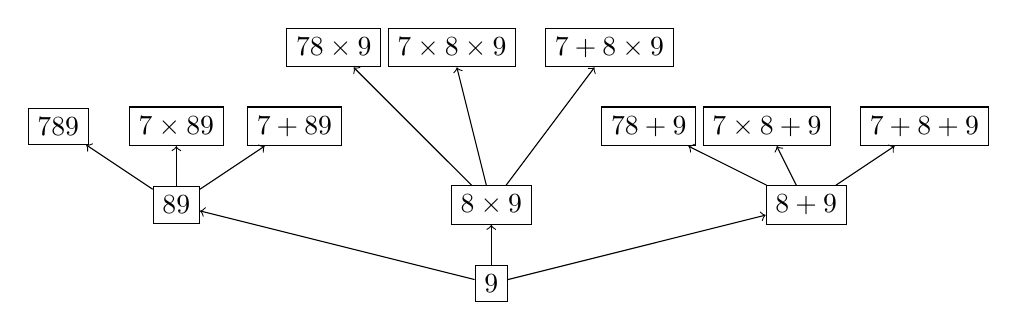
\begin{tikzpicture}
\path (0, 0)  node[rectangle, draw] (9) {9}
      (-4, 1) node[rectangle, draw] (89) {89}
      (0, 1)  node[rectangle, draw] (8x9) {$8 \times 9$}
      (4, 1)  node[rectangle, draw] (8+9) {$8 + 9$}
      (-5.5, 2) node[rectangle, draw] (789) {\sout{789}}
      (-4, 2) node[rectangle, draw] (7x89) {\sout{$7 \times 89$}}
      (-2.5, 2) node[rectangle, draw] (7+89) {$7 + 89$}
      (-2, 3) node[rectangle, draw] (78x9) {\sout{$78 \times 9$}}
      (-0.5, 3)  node[rectangle, draw] (7x8x9) {\sout{$7 \times 8 \times 9$}}
      (1.5, 3)  node[rectangle, draw] (7+8x9) {$7 + 8 \times 9$}
      (2, 2)  node[rectangle, draw] (78+9) {$78 + 9$}
      (3.5, 2)  node[rectangle, draw] (7x8+9) {$7 \times 8 + 9$}
      (5.5, 2)  node[rectangle, draw] (7+8+9) {$7 + 8 + 9$};
\draw[->] (9) edge (89)
          (9) edge (8x9)
          (9) edge (8+9)
          (89) edge (789)
          (89) edge (7x89)
          (89) edge (7+89)
          (8x9) edge (78x9)
          (8x9) edge (7x8x9)
          (8x9) edge (7+8x9)
          (8+9) edge (78+9)
          (8+9) edge (7x8+9)
          (8+9) edge (7+8+9);
\end{tikzpicture}
\caption{The process to expand expressions looks like a tree growing.}
\end{figure}

In order to evaluate the expression during expansion easily, we separate the value of the expression into 3 parts: the value of the first factor in the first sub-expression $f$; the product of the rest factors in the first sub-expression $v_{fs}$; and the sum of the rest sub-expressions $v_{ts}$. The overall value of the expression can be calculated out of them as $f \times v_{fs} + v_{ts}$.

When expand a new digit $d$ on the left, corresponding to the 3 options, the expression and value are updated as the following:

\begin{enumerate}
\item Insert nothing, prepend $d$ before the first factor as its most significant digit. The expression value is $(d \times 10^{n+1} + f) \times v_{fs} + v_{ts}$, where $n$ is the number of digits of $f$. The 3 parts of the value update to: $f' = d \times 10^{n+1} + f$, $v_{fs}$ and $v_{ts}$ are unchanged;

\item Insert $\times$, put $d$ as the first factor in the first sub-expression. The expression value is $d \times f \times v_{fs} + v_{ts}$. The 3 parts of the value update to: $f' = d, v_{fs'} = f \times v_{fs}$, while $v_{ts}$ is unchanged;

\item Insert +, use $d$ as the new first sub-expression. The expression value is $d + f \times v_{fs} + v_{ts}$. The 3 parts of the value update to: $f' = d, v_{fs'} = 1, v_{ts'} = f \times v_{fs} + v_{ts}$.
\end{enumerate}

To calculate $10^{n+1}$ in the first option easily, we can record the exponent as the fourth part of the expression value. As such, the value is represented as a 4-tuple $(e, f, v_{fs}, v_{ts})$. The function to calculate the value is defined as:

\be
value(e, f, v_{fs}, v_{ts}) = f \times v_{fs} + v_{ts}
\ee

When expand expression, we also update the 4-tuple at the same time:

\be
\begin{array}{rrl}
add & d\ (((ds:fs):ts), & (e, f, v_{fs}, v_{ts})) = \\
&  [(((d:ds):fs):ts, & (10 \times e, d \times e + f, v_{fs}, v_{ts})), \\
&   (([d]:ds:fs):ts, & (10, d, f \times v_{fs}, v_{ts})), \\
&   ([[d]]:(ds:fs):ts, & (10, d, 1, f \times v_{fs} + v_{ts}))] \\
\end{array}
\ee

For every expression and 4-tuple, we call $value$ function to calculate the value, drop it if exceeds 100. Then concatenate the candidate expressions and the 4-tuples to a list. According to this idea, we re-define the previous $extend$ function as below:

\be
\begin{cases}
expand\ d\ [] = [(expr(d), (10, d, 1, 0))] \\
expand\ d\ evs = concatMap\ ((filter\ ((\leq 100) \circ value \circ snd)) \circ (add\ d))\ evs\\
\end{cases}
\ee

We are ready to fold on $expand$, generate all candidate expressions and 4-tuples that do not exceed 100. Finally, we calculate the result from the 4-tuples, and leave only those equal to 100.

\be
map\ fst \circ filter\ ((=100) \circ value \circ snd)\ (foldr\ expand\ []\ [1, 2, ..., 9])
\ee

The complete program based on this definition is given in the appendix of this chapter. There are total 7 expressions evaluate to 100.

\[
\begin{array}{rl}
1: & 1 \times 2 \times 3 + 4 + 5 + 6 + 7 + 8 \times 9 \\
2: & 1 + 2 + 3 + 4 + 5 + 6 + 7 + 8 \times 9 \\
3: & 1 \times 2 \times 3 \times 4 + 5 + 6 + 7 \times 8 + 9 \\
4: & 12 + 3 \times 4 + 5 + 6 + 7 \times 8 + 9 \\
5: & 1 + 2 \times 3 + 4 + 5 + 67 + 8 + 9 \\
6: & 1 \times 2 + 34 + 5 + 6 \times 7 + 8 + 9 \\
7: & 12 + 34 + 5 \times 6 + 7 + 8 + 9 \\
\end{array}
\]

\begin{Exercise}
\Question{Use the fusion law to optimize the expression evaluation function:
\[
eval = sum \circ map\ (product \circ (map\ dec))
\]}
\Question{How to expand all expressions from left?}
\Question{The following definition converts expression to string:
\[
str = (join\ \text{``+''}) \circ (map\ ((join\ \text{``} \times \text{''}) \circ (map\ (show \circ dec))))
\]
Where $show$ converts number to string. Function $join(c, s)$ concatenates multiple strings $s$ with delimiter $c$. For example: $join($``\#''$, [$``abc'', ``def''$]) = $``abc\#def''. Use the fusion law to optimize $str$.
}
\end{Exercise}

\section{Further reading}

Program deduction is a special mathematical deduction. With this tool, we can start from intuitive, raw, and unoptimized definition, through a formalized methods and theorems, step by step convert it to elegant and optimized result. Bird gives many such examples in his {\em Pearls of Functional Algorithm Design}\cite{Bird-2010}.

The correctness of program deduction is based on mathematics. Instead of relying on human intuition, we need a dedicated theory, that can formalize varies of programs into strict mathematical form. The foldr/build fusion law is such an example. In the 1993 paper\cite{GLPJ-1993}, people developed a tool to simplify program systematically. As the category theory being widely adopted in programming, a series of fusion laws have been developed\cite{Hinze-Harper-James-2010}, and applied to program deduction and optimization.

\section{Appendix - example source code}

The \texttt{build} and \texttt{concatMap} definition in Haskell.

\lstset{frame=single}
\begin{lstlisting}
build :: forall a. (forall b. (a -> b -> b) -> b -> b) -> [a]
build g = g (:) []

concatMap f xs = build (\c n -> foldr (\x b -> foldr c b (f x)) n xs)
\end{lstlisting}

Exhaustive search solution for `Making a Century' puzzle:

\begin{lstlisting}
type Expr = [Term]     -- | T1 + T2 + ... Tn
type Term = [Factor]   -- | F1 * F2 * ... Fm
type Factor = [Int]    -- | d1d2...dk

dec :: Factor -> Int
dec = foldl (\n d -> n * 10 + d) 0

expr d = [[[d]]]  -- | single digit expr

eval [] = 0
eval (t:ts) = product (map dec t) + eval ts

extend :: Int -> [Expr] -> [Expr]
extend d [] = [expr d]
extend d es = concatMap (add d) es where
  add :: Int -> Expr -> [Expr]
  add d ((ds:fs):ts) = [((d:ds):fs):ts,
                        ([d]:ds:fs):ts,
                        [[d]]:(ds:fs):ts]

sol = filter ((==100) . eval) . foldr extend []
\end{lstlisting}

The improved exhaustive search solution:

\begin{lstlisting}
value (_, f, fs, ts) = f * fs + ts

expand d [] = [(expr d, (10, d, 1, 0))]
expand d evs = concatMap ((filter ((<= 100) . value . snd)) . (add d)) evs
where
  add d (((ds:fs):ts), (e, f, vfs, vts)) =
    [(((d:ds):fs):ts, (10 * e, d * e + f, vfs, vts)),
     (([d]:ds:fs):ts, (10, d, f * vfs, vts)),
     ([[d]]:(ds:fs):ts, (10, d, 1, f * vfs + vts))]

sol = map fst . filter ((==100) . value . snd) . foldr expand []
\end{lstlisting}

\ifx\wholebook\relax \else
\begin{thebibliography}{99}

\bibitem{GLPJ-1993}
Andrew Gill, John Launchbury, Simon L. Peyton Jones. ``A Short Cut to Deforestation''. Functional programming languages and computer architecture. pp. 223-232. 1993.

\bibitem{Bird-2010}
Richard Bird. ``Pearls of Functional Algorithm Design''. Cambridge University Press; 1 edition November 1, 2010. ISBN: 978-0521513388.

\bibitem{Hinze-Harper-James-2010}
Ralf Hinze, Thomas Harper, Daniel W. H. James. ``Theory and Practice of Fusion''. 2010, 22nd international symposium of IFL (Implementation and application of functional languages). pp.19-37.

\bibitem{Takano-Meijer-1995}
Akihiko Takano, Erik Meijer. ``Shortcut Deforestation in Calculational Form''. Functional programming languages and computer architecture. pp. 306-313. 1995.

\bibitem{Knuth-TAOCP-2006}
Donald Knuth. ``The Art of Computer Programming, Volume 4, Fascicle 4: Generating All Trees.'' Reading, MA: Addison-Wesley. ISBN: 978-0321637130. 2006.

\end{thebibliography}

\expandafter\enddocument
%\end{document}

\fi
